\chapter{Methodology}
\label{ch:methodology}

% ------------------------------------------------------------
\section{Overview of the Modelling Approach}
\label{sec:overview}
% ------------------------------------------------------------

This chapter presents the mathematical modeling and control design
methodology adopted for the semi-active energy-regenerative suspension
system under investigation. The system converts mechanical vibration
energy induced by road surface irregularities into electrical energy
stored in a battery while simultaneously attenuating body acceleration and tyre dynamic load
through semi-active force control. The complete plant comprises four
interconnected subsystems: a 2 DOF quarter-car suspension model with variable damping force, an equivalent circuit model of the motor and energy-regenerative
circuit, a unidirectional buck--boost power conversion stage with a
bridge rectifier, and a direct current controller consisting of a mode
decision module and a sliding mode controller.

Each subsystem is modelled using first-principles ordinary differential
equations (ODEs) derived from Newton's second law and Kirchhoff's
circuit laws. The subsystems are integrated into a unified nonlinear
state-space representation of the form

\begin{equation}
    \dot{\bm{x}}(t) = f\!\left(\bm{x}(t),\, u(t),\, d(t)\right)
    \label{eq:nonlinear_ss}
\end{equation}

where $\bm{x} \in \mathbb{R}^{4}$ is the state vector comprising the
mechanical states, $u \in [0,\,1]$ is the converter duty
cycle, and $d \in \mathbb{R}$ is the road surface displacement
disturbance. To regulate the system, a nested control architecture is
employed. In the outer loop, a model predictive controller determines the
optimal semi-active reference force required by the mechanical plant. This reference is then passed to the inner loop, where a sliding mode controller
computes the corresponding duty cycle to enforce robust current tracking
through the electrical converter dynamics. All numerical simulations are implemented in
MATLAB\textsuperscript{\textregistered}/Simulink using a
variable-step continuous solver appropriate for the multi-timescale
dynamics of the combined mechanical--electrical plant.



% ------------------------------------------------------------
\section{State Vector and Signal Definitions}
\label{sec:state_vector}
% ------------------------------------------------------------

The system state vector is defined as

\begin{equation}
    \bm{x} =
    \begin{bmatrix}
        x_1 & x_2 & x_3 & x_4
    \end{bmatrix}^{\!\top}
    \label{eq:state_vector}
\end{equation}

where each state corresponds to a physically meaningful quantity as
summarised in \cref{tab:states}.

\begin{table}[htbp]
    \centering
    \caption{Definition of system states}
    \label{tab:states}
    \renewcommand{\arraystretch}{1.35}
    \begin{tabular}{clll}
        \toprule
        State & Symbol & Description & Unit \\
        \midrule
        $x_1$ & $z_s$       & Sprung mass (body) displacement    & \si{\metre}            \\
        $x_2$ & $\dot{z}_s$ & Sprung mass velocity               & \si{\metre\per\second} \\
        $x_3$ & $z_u$       & Unsprung mass (wheel) displacement & \si{\metre}            \\
        $x_4$ & $\dot{z}_u$ & Unsprung mass velocity             & \si{\metre\per\second} \\
        \bottomrule
    \end{tabular}
\end{table}

The electrical states $i_L$ (inductor current) and $E_C$ (battery
terminal voltage) are treated separately from the mechanical state
vector. In this study the battery terminal voltage is assumed constant,
$E_C = E_r = \SI{12}{\volt}$, consistent with the stiff battery
approximation valid over the timescale of the suspension dynamics.
Under this assumption the electrical subsystem reduces to a single
first-order ODE in $i_L$. The control input and disturbance signal of the mechanical states are
defined as

\begin{equation}
    u = F, \qquad d = z_r
    \label{eq:inputs}
\end{equation}

where $F$ is the variable damping force and $z_r(t)$ [\si{\metre}] is
the road surface displacement. The measured output vector is

\begin{equation}
    \bm{y} =
    \begin{bmatrix}
        \ddot{z}_s & F_{t}
    \end{bmatrix}^{\!\top}
    \label{eq:outputs}
\end{equation}

comprising body acceleration (comfort metric) and tyre dynamic load (performance metric). The power generated $P$ is also calculated externally and taken as a metric.

% ------------------------------------------------------------
\section{Subsystem Models}
\label{sec:subsystems}
% ------------------------------------------------------------

\subsection{Quarter-Car Suspension Model}
\label{subsec:quarter_car}

The suspension is represented by the classical two-degree-of-freedom
(2-DOF) quarter-car model, which captures the dominant vertical dynamics
of a single corner of the vehicle. The model comprises two lumped
masses: the sprung mass $m_s$ (vehicle body) and the unsprung mass
$m_u$ (wheel--axle assembly), coupled by the suspension spring $k_s$
and the linear motor actuator. The tyre is modelled as a linear spring
$k_t$ connecting the unsprung mass to the road surface, with the tyre
damping assumed negligible.

Applying Newton's second law to each mass yields

\begin{align}
    m_s\,\ddot{z}_s &=
        -k_s(z_s - z_u) + F
        \label{eq:sprung_mass}\\[6pt]
    m_u\,\ddot{z}_u &=
        \phantom{-}k_s(z_s - z_u)
        - k_t(z_u - z_r)
        - F
        \label{eq:unsprung_mass}
\end{align}

where $F = k_i\,i_L$ is the electromagnetic damping force produced by
the linear motor, $k_i$ [\si{\newton\per\ampere}] is the motor thrust
constant, and $i_L$ is the motor winding current. The passivity
constraint $F\,(\dot{z}_s - \dot{z}_u) \geq 0$ must hold during
energy-regenerative operation, since the linear motor operates as a
generator and cannot inject mechanical energy into the suspension under
the proposed control strategy. The nominal suspension parameters used
in this study are listed in \cref{tab:qcar_params}.

\begin{table}[htbp]
    \centering
    \caption{Quarter-car model parameters}
    \label{tab:qcar_params}
    \renewcommand{\arraystretch}{1.3}
    \begin{tabular}{llll}
        \toprule
        Parameter & Symbol & Value & Unit \\
        \midrule
        Sprung mass          & $m_s$ & 82      & \si{\kilogram} \\
        Unsprung mass        & $m_u$ & 11.5    & \si{\kilogram} \\
        Suspension stiffness & $k_s$ & 5{,}495 & \si{\newton\per\metre} \\
        Tyre stiffness       & $k_t$ & 48{,}000 & \si{\newton\per\metre} \\
        \bottomrule
    \end{tabular}
\end{table}

\subsection{Linear Motor and Equivalent Circuit Model}
\label{subsec:motor}

The linear motor operates as an electromagnetic generator, converting
relative suspension motion into electrical energy. Its back
electromotive force (EMF) and winding current are governed by

\begin{equation}
    E = k_e\, v, \qquad v = \dot{z}_s - \dot{z}_u
    \label{eq:emf}
\end{equation}

\begin{equation}
    F = k_i\, i_L
    \label{eq:force}
\end{equation}

where $k_e$ [\si{\volt\second\per\metre}] is the back-EMF constant,
$v$ is the relative velocity across the suspension, and $k_i$
[\si{\newton\per\ampere}] is the motor thrust constant. The maximum
winding current achievable when the motor terminals are directly
connected is

\begin{equation}
    i_{max} = \frac{E}{R} = \frac{k_e\,|v|}{R}
    \label{eq:imax}
\end{equation}

and the corresponding maximum electromagnetic damping force is

\begin{equation}
    F_{max} = \frac{k_i\,k_e}{R}\,|v| = c_e\,|v|
    \label{eq:fmax}
\end{equation}

where $c_e = k_i k_e / R$ [\si{\newton\second\per\metre}] is the motor
damping coefficient and $R$ is the winding resistance. The tracking
constant $\alpha$, which describes the ratio of the required control
force to the maximum available force, is defined as

\begin{equation}
    \alpha = \left|\frac{F_{ref}}{F_{max}}\right| \leq 1
    \label{eq:alpha}
\end{equation}

When $\alpha \leq 1$ the desired force lies within the controllable
region and semi-active control is realisable. When $\alpha > 1$ the
required force exceeds the generator capability and the motor is
controlled to operate as a passive electromagnetic damper.

\subsection{Energy-Regenerative Circuit}
\label{subsec:circuit}

The energy-regenerative circuit comprises a diode bridge rectifier
followed by a unidirectional boost--buck converter, as shown
schematically in \cref{fig:circuit}. The bridge rectifier ensures that
the converter input voltage and inductor current are always non-negative,
regardless of the direction of motor motion. This allows a single
averaged converter model to represent both directions of suspension
travel. The converter operates in one of three modes depending on the
instantaneous motor velocity and required current:

\begin{itemize}
    \item \textbf{Boost mode}: transistor VT1 held on, VT2 provided
          with PWM signal. The converter steps up the motor EMF to
          overcome the battery voltage, increasing the winding current.
    \item \textbf{Buck mode}: transistor VT2 held on, VT1 provided
          with PWM signal. The converter steps down the effective
          voltage, decreasing the winding current.
    \item \textbf{Passive mode}: both VT1 and VT2 switched on
          simultaneously. The battery is open-circuited and the motor
          windings are directly connected, producing the maximum passive
          electromagnetic damping force $F_{max}$.
\end{itemize}
\begin{figure}
    \centering
    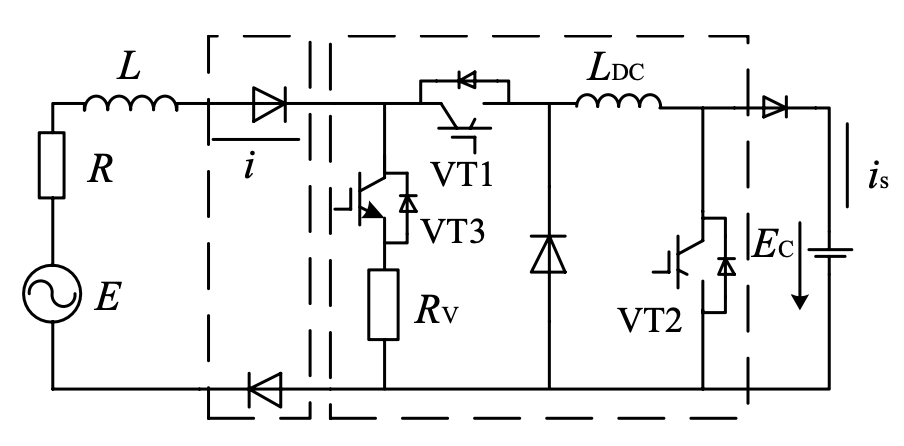
\includegraphics[width=0.5\linewidth]{Thesis Pictures/unidirectional.png}
    \caption{Uni-directional buck-boost converter topology}
    \label{fig:unidirectional}
\end{figure}
\subsubsection{Boost Mode KVL Analysis}
\label{subsubsec:boost_kvl}

In boost mode VT1 is held on and VT2 is switched with duty cycle $D$
and period $T$. Two sub-intervals are identified within each switching
period.

\textbf{Sub-interval 1} $(0 < t \leq t_{on} = DT)$: VT2 is on and
the battery is open-circuited. Applying KVL around the motor--inductor
loop gives

\begin{equation}
    (L + L_{DC})\frac{di}{dt} + iR = E
    \label{eq:boost_on}
\end{equation}

With initial current $I_{10}$ the solution is

\begin{equation}
    i_1(t) = I_{10}\,e^{-t/\tau}
             + \frac{E}{R}\!\left(1 - e^{-t/\tau}\right), \qquad
    \tau = \frac{L + L_{DC}}{R}
    \label{eq:boost_i1}
\end{equation}

\textbf{Sub-interval 2} $(t_{on} < t \leq T)$: VT2 is off and the
motor charges the battery directly. KVL gives

\begin{equation}
    (L + L_{DC})\frac{di}{dt} + iR + E_C = E
    \label{eq:boost_off}
\end{equation}

With initial current $I_{20} = i_1(DT)$ the solution is

\begin{equation}
    i_2(t) = I_{20}\,e^{-(t-DT)/\tau}
             + \frac{E - E_C}{R}
               \!\left(1 - e^{-(t-DT)/\tau}\right)
    \label{eq:boost_i2}
\end{equation}

Under CCM the current is periodic, so $I_{10} = i_2(T)$. Applying
this boundary condition to \cref{eq:boost_i1,eq:boost_i2} and solving
for $I_{10}$ and $I_{20}$ yields

\begin{equation}
    I_{10} = \frac{E}{R}
             - \frac{E_C}{R}
               \cdot\frac{1 - e^{-(1-D)T/\tau}}{1 - e^{-T/\tau}}
               \cdot e^{-DT/\tau}
    \label{eq:boost_I10}
\end{equation}

\begin{equation}
    I_{20} = \frac{E}{R}
             - \frac{E_C}{R}
               \cdot\frac{1 - e^{-(1-D)T/\tau}}{1 - e^{-T/\tau}}
    \label{eq:boost_I20}
\end{equation}

\subsubsection{Buck Mode KVL Analysis}
\label{subsubsec:buck_kvl}

In buck mode VT2 is held on and VT1 is switched with duty cycle $D$.
Two sub-intervals are again identified.

\textbf{Sub-interval 1} $(0 < t \leq DT)$: VT1 is on and the winding
current flows through the battery. KVL gives

\begin{equation}
    (L + L_{DC})\frac{di}{dt} + iR + E_C = E
    \label{eq:buck_on}
\end{equation}

With initial current $I_{10}$ the solution is

\begin{equation}
    i_1(t) = I_{10}\,e^{-t/\tau}
             + \frac{E - E_C}{R}
               \!\left(1 - e^{-t/\tau}\right)
    \label{eq:buck_i1}
\end{equation}

\textbf{Sub-interval 2} $(DT < t \leq T)$: VT1 is off. The stored
inductive energy continues to drive current through the freewheeling
path via the converter resistance $R_V$. KVL gives

\begin{equation}
    L\frac{di}{dt} + i(R + R_V) = E
    \label{eq:buck_off}
\end{equation}

with time constant $\tau_V = L/(R + R_V)$. With initial current
$I_{20} = i_1(DT)$

\begin{equation}
    i_2(t) = I_{20}\,e^{-(t-DT)/\tau_V}
             + \frac{E}{R + R_V}
               \!\left(1 - e^{-(t-DT)/\tau_V}\right)
    \label{eq:buck_i2}
\end{equation}

Applying the CCM periodicity condition $I_{10} = i_2(T)$ and solving
yields expressions for $I_{10}$ and $I_{20}$ analogous to
\cref{eq:boost_I10,eq:boost_I20}.

\subsubsection{Steady-State Current Under CCM Averaging}
\label{subsubsec:ccm_avg}

For switching periods $T$ much smaller than the mechanical time
constant $\tau_s = 2m_s/c_e$, the exponential terms in
\cref{eq:boost_i1,eq:boost_i2,eq:buck_i1,eq:buck_i2} may be
expanded to first order via the Taylor approximation
$e^{-x} \approx 1 - x$ for $x \ll 1$. Under this approximation
the periodic boundary conditions reduce to algebraic expressions
for the average steady-state winding current.

For boost mode the average steady-state current is

\begin{equation}
    \bar{I}_{boost} =
        \frac{E - (1-D)\,E_C}{R}
    \label{eq:Iboost}
\end{equation}

For buck mode the average steady-state current is

\begin{equation}
    \bar{I}_{buck} =
        \frac{E - D\,E_C}{R + R_V - D\,R_V}
    \label{eq:Ibuck}
\end{equation}

These expressions define the attainable current range in each
operating mode as a function of duty cycle $D \in [0,\,1]$, motor
EMF $E$, and battery voltage $E_C$. The variation ranges are
summarised in \cref{tab:current_range} and provide the theoretical
basis for the mode decision law described in \cref{subsec:mode}.

\begin{table}[htbp]
    \centering
    \caption{Variation range of winding current in each operating mode}
    \label{tab:current_range}
    \renewcommand{\arraystretch}{1.3}
    \begin{tabular}{lll}
        \toprule
        Mode    & Condition      & Current range $i$ \\
        \midrule
        Boost   & $E > E_C$
                & $\dfrac{E - E_C}{R} \leq i < \dfrac{E}{R}$ \\[8pt]
        Buck    & $E > E_C$
                & $\dfrac{E}{R+R_V} \leq i < \dfrac{E-E_C}{R}$ \\[8pt]
        None    & $E \leq E_C$   & $0 \leq i < E/R$ \\
        \bottomrule
    \end{tabular}
\end{table}

\subsubsection{Averaged State Equations}
\label{subsubsec:avg_state}

Replacing the switched circuit variables with their cycle-averaged
equivalents and substituting \cref{eq:Iboost,eq:Ibuck} into the
respective KVL expressions, the averaged state equation for the
inductor current across all three operating modes is

\begin{equation}
\resizebox{\linewidth}{!}{$
    \dot{i}_L =
    \begin{cases}
        \displaystyle
        -\frac{R}{L+L_{DC}}\,i_L -\frac{1-D}{L+L_{DC}}\,E_C +\frac{1}{L+L_{DC}}\,E 
        & \text{boost}\\[15pt]
        \displaystyle
        -\frac{DRL+(1-D)(R+R_V)(L+L_{DC})}{L(L+L_{DC})}\,i_L -\frac{D}{L+L_{DC}}\,E_C +\frac{DL+(1-D)(L+L_{DC})}{L(L+L_{DC})}\,E 
        & \text{buck}\\[15pt]
        \displaystyle
        -\frac{R}{L+L_{DC}}\,i_L +\frac{1}{L+L_{DC}}\,E 
        & \text{passive}
    \end{cases}
$}
\label{eq:diL}
\end{equation}

where $L$ is the winding inductance, $L_{DC}$ is the converter
inductance, $R_V$ is the converter resistance, $E_C$ is the battery
terminal voltage, $E = k_e\,|v|$ is the rectified motor EMF, and
$D \in [0,\,1]$ is the duty cycle. In passive mode the battery is
open-circuited; accordingly the $E_C$ term is absent and $D$ is
replaced by unity. The motor and circuit parameters are listed in
\cref{tab:motor_params}.

\begin{table}[htbp]
    \centering
    \caption{Linear motor and circuit parameters}
    \label{tab:motor_params}
    \renewcommand{\arraystretch}{1.3}
    \begin{tabular}{llll}
        \toprule
        Parameter & Symbol & Value & Unit \\
        \midrule
        Winding resistance    & $R$    & 10.2  & \si{\ohm}              \\
        Winding inductance    & $L$    & 12.8  & \si{\milli\henry}      \\
        Thrust constant       & $k_i$  & 77.9  & \si{\newton\per\ampere}\\
        Back-EMF constant     & $k_e$  & 62.6  
            & \si{\volt\second\per\metre}                               \\
        Battery voltage       & $E_r$  & 12    & \si{\volt}             \\
        Converter resistance  & $R_V$  & 10.2  & \si{\ohm}              \\
        \bottomrule
    \end{tabular}
\end{table}

\section{Cascaded Control Architecture}
\label{sec:cascaded_topology}

The complete energy-regenerative suspension system is governed by a cascaded (or nested) control topology. This multi-loop architecture is deliberately chosen to address the multi-timescale nature of the plant, decoupling the relatively slow mechanical dynamics of the quarter-car suspension from the highly nonlinear, high-frequency switching dynamics of the unidirectional boost--buck power converter. 

The cascaded topology is divided into two primary loops: an outer mechanical control loop and an inner electrical tracking loop, bridged by an intermediate mode decision interface.

\subsection{Outer Loop: High-Level Force Optimization}
The outer loop is responsible for the macroscopic dynamic performance of the vehicle. It operates on the mechanical time scale (sampled at $T_s = \SI{5}{\milli\second}$) and assumes the electrical actuator acts as an ideal force generator. In this framework, the Model Predictive Controller (MPC) acts as the high-level supervisor. By measuring the mechanical state vector—comprising sprung and unsprung mass displacements and velocities—the MPC solves a finite-horizon optimization problem. It continuously evaluates the trade-off between ride comfort and road holding, utilizing the adaptive velocity-dependent scheduling strategy to compute the optimal target damping force, $F_{ref}$.

\subsection{Intermediate Interface: Mode Decision and Current Mapping}
Because the electromagnetic motor is fundamentally an electrical machine, the optimal mechanical force $F_{ref}$ cannot be commanded directly; it must be translated into an electrical reference. The intermediate interface handles this translation by converting the reference force into a target inductor current, $i_{ref}$, via the motor's thrust constant. 

Simultaneously, the mode decision module evaluates the instantaneous motor velocity and back-electromotive force (EMF) against the battery voltage. Based on the fundamental passivity constraint ($\alpha \le 1$), it determines the required structural mode of the power converter: boost mode (to step up the EMF), buck mode (to step down the voltage), or passive mode (if the requested force exceeds generation capacity). This ensures that the downstream electrical controller always receives physically feasible targets.

\subsection{Inner Loop: Low-Level Current Tracking}
The inner loop handles the microscopic electrical dynamics, operating at a much higher frequency than the outer loop to manage the pulse-width modulation (PWM) switching. The Sliding Mode Controller (SMC) drives this inner loop. It receives the target current $i_{ref}$ and the structural mode decision from the intermediate interface, continuously comparing them against the actual measured inductor current, $i_L$. 

By defining a distinct sliding surface for both the buck and boost operating regions, the SMC robustly computes the exact duty cycle required to track $i_{ref}$. This nested approach ensures that any high-frequency electrical disturbances, parameter uncertainties in the winding resistance, or variations in the battery state-of-charge are rapidly rejected by the inner loop before they can propagate outward and degrade the mechanical ride quality.

\begin{figure}[H]
    \centering
    \resizebox{\textwidth}{!}{% Resizes the diagram to perfectly fit page margins
    \begin{tikzpicture}[
        >=latex,
        auto,
        node distance=3.5cm and 2.5cm,
        block/.style={rectangle, draw=black, thick, fill=white, text width=3.2cm, align=center, rounded corners=3pt, minimum height=1.5cm},
        dashbox/.style={draw, dashed, thick, inner sep=12pt, rounded corners=5pt}
    ]

    % 1. Place the controller nodes (Top Row)
    \node[block] (mpc) {Model Predictive\\Controller (MPC)};
    \node[block, above=0.8cm of mpc, fill=blue!5] (scheduler) {Adaptive Weight\\Scheduler};
    \node[block, right=of mpc] (interface) {Mode Decision \&\\Current Mapping};
    \node[block, right=of interface] (smc) {Sliding Mode\\Controller (SMC)};

    % 2. Place the plant nodes (Bottom Row)
    \node[block, below=2cm of smc, fill=gray!10] (converter) {Boost-Buck\\Converter};
    \node[block, left=of converter, fill=gray!10] (motor) {Linear Electro-\\magnetic Motor};
    \node[block, left=of motor, fill=gray!10] (qcar) {Quarter-Car\\Suspension};

    % 3. Draw dashed grouping boxes using 'fit'
    \begin{scope}[on background layer]
        % Outer Loop Box
        \node[dashbox, fill=blue!2, fit=(scheduler) (mpc)] (outerloop) {};
        \node[above left, inner sep=2pt, text=blue!80!black, font=\small\bfseries] at (outerloop.north west) {Outer Control Loop};

        % Plant Box
        \node[dashbox, fill=green!2, fit=(converter) (motor) (qcar)] (plant) {};
        \node[below left, inner sep=2pt, text=green!60!black, font=\small\bfseries] at (plant.south west) {Electro-Mechanical Plant};
    \end{scope}

    % 4. Draw connecting arrows
    % Inputs to Scheduler
    \coordinate (vx_in) at ($(scheduler.west) + (-1.5,0)$);
    \draw[->, thick] (vx_in) -- node[above] {Speed $v_x$} (scheduler.west);

    % Scheduler to MPC
    \draw[->, thick] (scheduler.south) -- node[right] {$w_c, w_r$} (mpc.north);

    % MPC to Interface
    \draw[->, thick] (mpc.east) -- node[above] {$F_{ref}$} (interface.west);

    % Interface to SMC
    \draw[->, thick] (interface.east) -- node[above] {$i_{ref}$, Mode} (smc.west);

    % SMC to Converter (Down)
    \draw[->, thick, transform canvas={xshift=-0.5cm}] (smc.south) -- node[left] {Duty $D$} (converter.north);

    % Converter to SMC Feedback (Up)
    \draw[<-, thick, transform canvas={xshift=0.5cm}] (smc.south) -- node[right] {$i_L$} (converter.north);

    % Converter to Motor (Leftwards)
    \draw[->, thick, transform canvas={yshift=0.3cm}] (converter.west) -- node[above] {$i_L$} (motor.east);
    \draw[<-, thick, transform canvas={yshift=-0.3cm}] (converter.west) -- node[below] {EMF $E$} (motor.east);

    % Motor to QCar (Leftwards)
    \draw[->, thick, transform canvas={yshift=0.3cm}] (motor.west) -- node[above] {$F_{act}$} (qcar.east);
    \draw[<-, thick, transform canvas={yshift=-0.3cm}] (motor.west) -- node[below] {Vel. $v$} (qcar.east);

    % Feedbacks to Controllers (Upwards)
    \draw[->, thick] (qcar.north) -- node[left] {States $\bm{x}$} (mpc.south);
    \draw[->, thick] (motor.north) -- node[left] {Vel. $v$} (interface.south);

    % External Inputs & Outputs
    \coordinate (road_in) at ($(qcar.south) + (0,-1.2)$);
    \draw[->, thick] (road_in) -- node[right] {Road Profile $z_r$} (qcar.south);

    \coordinate (metrics_out) at ($(qcar.west) + (-1.5,0)$);
    \draw[->, thick] (qcar.west) -- node[above] {$\ddot{z}_s, F_t$} (metrics_out);

    \coordinate (power_out) at ($(converter.east) + (1.5,0)$);
    \draw[->, thick] (converter.east) -- node[above] {Power $P$} (power_out);

    \end{tikzpicture}
    }
    \caption{Block diagram of the cascaded control topology, illustrating the outer-loop MPC, intermediate mode decision, inner-loop SMC, and the electro-mechanical plant.}
    \label{fig:cascaded_topology}
\end{figure}

Ultimately, this modular separation of concerns guarantees structural stability. It allows the complex optimization of ride comfort and road holding to be computed independently of the nonlinear converter switching, enabling both controllers to operate at their respective ideal bandwidths.



% ------------------------------------------------------------
\section{Semi-Active Control Strategy}
\label{sec:semi_active}
% ------------------------------------------------------------

\subsection{Skyhook-Groundhook Reference Force Generation}
\label{subsec:frefsg}

The reference electromagnetic force is derived from a combined
skyhook--groundhook control law, which simultaneously targets ride
comfort and road-holding performance. The skyhook component damps
absolute body motion, while the groundhook component damps absolute
wheel motion. The reference force is given by

\begin{equation}
    F_{ref} = -c_s\,\dot{z}_s - c_g\,\dot{z}_u
    \label{eq:fref}
\end{equation}

where $c_s \geq 0$ and $c_g \leq 0$ are the skyhook and groundhook
gain coefficients respectively. These are expressed as

\begin{equation}
    c_s = m\,c_e, \qquad c_g = -n\,c_s
    \label{eq:gains}
\end{equation}

where $m > 0$ and $n > 0$ are dimensionless tuning parameters and
$c_e = k_i k_e / R$ is the motor damping coefficient. The stability
of the energy-regenerative suspension requires $c_s > 0$ and
$c_g \leq 0$. The parameters $m = 1.45$ and $n = 0.39$
are selected. The reference current is obtained by inverting \cref{eq:force}:

\begin{equation}
    i_{ref} = \frac{|F_{ref}|}{k_i}
    \label{eq:iref}
\end{equation}

The absolute value is taken because the bridge rectifier constrains
the inductor current to be non-negative; the sign of the actual
electromagnetic force is recovered at the output by

\begin{equation}
    F_{act} = k_i\,i_L\,\mathrm{sgn}(v)
    \label{eq:fact}
\end{equation}

which restores the correct force direction consistent with the
physical motor convention.

\subsection{Model Predictive Force Reference Generation}
\label{subsec:frefmpc}

% ------------------------------------------------------------

The skyhook--groundhook control law described in \cref{subsec:frefsg}
computes the reference force $F_{ref}$ as a static, memoryless function
of the instantaneous suspension velocities. While this approach is
computationally efficient and analytically tractable, it does not
explicitly account for the competing
objectives of ride comfort and road holding in a unified optimisation
framework.

Model predictive control (MPC) offers a principled alternative in which
the reference force is computed by solving a constrained finite-horizon
optimisation problem at each sampling instant. By incorporating
the suspension dynamics into the formulation,
the MPC produces a reference force that optimally balances ride comfort
and road holding. The MPC replaces only the force reference
generator; the downstream mode decision module and sliding mode current
controller described in \cref{subsec:mode,sec:smc} remain unchanged.
\begin{figure}
    \centering
    
\includegraphics[width=0.5\linewidth]{Thesis Pictures/mpc.png}
    \caption{MPC operating principle}
    \label{fig:mpc}
\end{figure}
\subsubsection{Prediction Model}
\label{subsubsec:mpc_model}

The MPC operates on a discrete-time linearisation of the quarter-car
suspension model. Defining the state vector as

\begin{equation}
    \bm{x}_k =
    \begin{bmatrix}
        z_s & \dot{z}_s & z_u & \dot{z}_u
    \end{bmatrix}_k^{\!\top}
    \label{eq:mpc_state}
\end{equation}

and the control input as the reference electromagnetic force
$u_k = F_{ref,k}$, the continuous-time equations
\cref{eq:sprung_mass,eq:unsprung_mass} are discretised using the
zero-order hold (ZOH) method at sampling period $T_s = \SI{5}{\milli\second}$,
yielding

\begin{equation}
    \bm{x}_{k+1} = A_d\,\bm{x}_k + B_d\,u_k + E_d\,z_{r,k}
    \label{eq:mpc_discrete}
\end{equation}

where the discrete system matrices are

\begin{equation}
    A_d = e^{A_c T_s}, \quad
    B_d = \int_0^{T_s} e^{A_c \tau}\,B_c\,\mathrm{d}\tau, \quad
    E_d = \int_0^{T_s} e^{A_c \tau}\,E_c\,\mathrm{d}\tau
    \label{eq:zoh}
\end{equation}

and the continuous-time matrices are

\begin{equation}
    A_c =
    \begin{bmatrix}
        0 & 1 & 0 & 0 \\
        -k_s/m_s & 0 & k_s/m_s & 0 \\
        0 & 0 & 0 & 1 \\
        k_s/m_u & 0 & -(k_s+k_t)/m_u & 0
    \end{bmatrix}, \quad
    B_c =
    \begin{bmatrix}
        0 \\ 1/m_s \\ 0 \\ -1/m_u
    \end{bmatrix}, \quad
    E_c =
    \begin{bmatrix}
        0 \\ 0 \\ 0 \\ k_t/m_u
    \end{bmatrix}
    \label{eq:continuous_matrices}
\end{equation}

The road disturbance $z_{r,k}$ is treated as a measured disturbance
and assumed constant over the prediction horizon, consistent with the
receding-horizon approximation.

\subsubsection{Prediction Horizon}\label{subsubsec:mpc_horizon}The prediction horizon $N_p$ and control horizon $N_c$ are selected to balance closed-loop performance against computational burden. The dominant mechanical time constant of the sprung mass is $\tau_s = 2m_s / c_e \approx \SI{0.34}{\second}$, corresponding to approximately 68 sampling steps at $T_s = \SI{5}{\milli\second}$. A prediction horizon of $N_p = 120$ steps (\SI{600}{\milli\second}) is selected to sufficiently capture the dominant sprung mass transient dynamics while remaining computationally tractable for real-time implementation. A control horizon of $N_c = 4$ steps is used, with the remaining $N_p - N_c$ steps held constant at the last optimised value. These values are consistent with MPC horizon selections reported in the suspension control literature and are summarised in \cref{tab:mpc_params}.

\subsubsection{Cost Function}\label{subsubsec:mpc_cost}The MPC cost function is formulated to simultaneously minimise body acceleration (ride comfort) and tyre dynamic load (road holding).The finite-horizon cost is 
\begin{equation}
    J = \sum_{j=1}^{N_p}
    \left[
        w_c\,\ddot{z}_{s,k+j}^2
        + w_r\,\left(k_t(z_{u,k+j} - z_{r,k})\right)^2
    \right]
    + \sum_{j=0}^{N_c-1} w_{\Delta u}\,\Delta u_{k+j}^2
    \label{eq:mpc_cost}
\end{equation}
where the three terms represent, respectively, the body acceleration penalty (comfort), the tyre dynamic load penalty (road holding),and the control increment penalty (actuator smoothness). The weights $w_c \geq 0$, $w_r \geq 0$, and $w_{\Delta u} \geq 0$ are tuning parameters whose relative magnitudes determine the trade-off between these objectives. The control increment $\Delta u_{k+j} = u_{k+j} -
u_{k+j-1}$ penalizes rapid changes in the reference force, which would otherwise excite high-frequency switching in the downstream SMC. The body acceleration appearing in the comfort term is expressed as a linear function of the states and input using \cref{eq:sprung_mass}:\begin{equation}\ddot{z}{s,k+j} = \frac{-k_s(z{s,k+j} - z_{u,k+j}) + u_{k+j}}{m_s}\label{eq:zdds}\end{equation}The nominal weight values used in this study are listed in\cref{tab:scheduling_params}. These are selected such that the comfort and road-holding terms are of comparable magnitude at the sprung and unsprung mass resonance frequencies.

\subsubsection{Constraints}\label{subsubsec:mpc_constraints}Two classes of constraints are imposed at each prediction step $j = 0, \ldots, N_c - 1 $: \newline
\textbf{Dead-zone constraint.} No reference force is commanded when the motor velocity falls below the critical threshold:\begin{equation}u_{k+j} = 0 \quad \text{if } |v_k| < v_d = E_C / k_e\label{eq:constraint_deadzone}\end{equation}\textbf{Control increment constraint.} The rate of change of the reference force is bounded to prevent impulsive demands on the downstream SMC:\begin{equation}|\Delta u_{k+j}| \leq \Delta F_{max}\label{eq:constraint_rate}\end{equation}where $\Delta F_{max} = \SI{50}{\newton}$ per sample, correspondingto a maximum force slew rate of \SI{10}{\kilo\newton\per\second}.Together, \cref{eq:constraint_deadzone,eq:constraint_rate} define a convex feasible set for the optimisation at each sampling instant. The resulting quadratic programme (QP) is solved using the MATLAB \texttt{quadprog} solver at each time step, with warm-starting from the previous solution to reduce computation time.
\subsubsection{Receding Horizon Implementation}
\label{subsubsec:mpc_receding}

At each sampling instant $k$, the MPC executes the following steps:

\begin{enumerate}
    \item Measure the current state $\bm{x}_k = [z_s,\,\dot{z}_s,\,z_u,\,\dot{z}_u]_k^\top$
          from the quarter-car subsystem.
    \item Compute $F_{max,k} = c_e\,|v_k|$, $v_d = E_C/k_e$, and
          $\alpha_k = |F_{ref,k-1}|/F_{max,k}$ from the previous
          reference force.
    \item If $|v_k| < v_d$, set $F_{ref,k} = 0$ and skip the QP.
    \item Otherwise, solve the QP defined by \cref{eq:mpc_cost}
          subject to \cref{eq:constraint_rate,eq:constraint_deadzone}
          over the prediction horizon $N_p$ using the discrete model
          \cref{eq:mpc_discrete}.
    \item Apply only the first element of the optimal control sequence:
          $F_{ref,k} = u_k^\star$.
    \item Convert to reference current: $i_{ref,k} = |F_{ref,k}|/k_i$.
    \item Pass $F_{ref,k}$, $i_{ref,k}$, and $\alpha_k$ to the mode
          decision module and SMC.
\end{enumerate}

The receding-horizon principle ensures recursive feasibility: provided
the initial state is feasible, the constraint set remains non-empty
at all subsequent steps because $F_{ref} = 0$ is always a feasible
solution.
\subsubsection{Weight Selection and Trade-off Analysis}\label{subsubsec:mpc_weights}The MPC weights $w_c$, $w_r$, and $w_{\Delta u}$are the primary tuning parameters of the controller. Their physical interpretation is as follows:\begin{itemize}\item $w_c$ governs the emphasis on ride comfort. Increasing $w_c$ reduces body acceleration at the cost of larger tyre dynamic loads.\item $w_r$ governs the emphasis on road holding. Increasing $w_r$ reduces tyre lift-off probability at the cost of increased body acceleration.\item $w_{\Delta u}$ governs actuator smoothness. Increasing $w_{\Delta u}$ reduces force rate-of-change at the cost of slower reference tracking.\end{itemize}In conventional MPC formulations, these weights are often held constant or manually toggled between discrete driving modes. However, because ride comfort and road holding are fundamentally competing objectives, a fixed weight combination inevitably compromises performance across varying driving conditions. To resolve this, the proposed architecture employs an adaptive weight scheduling strategy based on the vehicle's longitudinal speed.
\subsection{Adaptive Weight Scheduling}\label{subsec:mpc_scheduling}The rationale for utilizing longitudinal vehicle speed as a scheduling variable lies in its direct relationship to the road excitation spectrum. Driving speed serves as a highly effective, instantaneously measurable proxy for the dominant temporal frequency band experienced by the suspension. At low speeds, the spatial frequencies of standard road irregularities primarily translate into low-frequency temporal excitations, placing the vehicle predominantly within the sprung mass resonance regime ($\sim\SI{1.3}{\hertz}$). At high speeds, the same spatial road profile shifts the temporal excitation into a substantially higher frequency band, increasingly exciting the unsprung mass resonance ($\sim\SI{10.9}{\hertz}$) and demanding greater dynamic tyre control.
At low driving speeds, the dynamic forces acting on the tyre are generally small, providing a large safety margin for road holding. This allows the controller to safely prioritise passenger comfort. Conversely, at high speeds, aerodynamic effects and severe road impacts make maintaining continuous tyre-road contact critical for vehicle stability and safety, necessitating a shift in priority toward road holding.To achieve a seamless transition between these two paradigms, the penalty weights $w_c$ (comfort) and $w_r$ (road holding) are dynamically updated at runtime using a sigmoid-based scheduling function dependent on the longitudinal vehicle speed $v_x$. A dimensionless scheduling parameter $\alpha \in (0,\,1)$ is defined by the logistic function:\begin{equation}\alpha(v_x) = 1 - \frac{1}{1 + e^{-k(v_x - v_{mid})}}\label{eq:sigmoid_alpha}\end{equation}where $v_{mid}$ is the inflection point representing a balanced 50/50 focus between comfort and performance, and $k$ dictates the steepness of the transition region. For this implementation, the inflection speed is set to $v_{mid} = \SI{50}{\kilo\metre\per\hour}$ with a transition steepness of $k = 0.3$. As a result, $\alpha \to 1$ at low speeds (pure comfort focus) and $\alpha \to 0$ at high speeds (pure performance focus). The instantaneous MPC weights are then computed via linear interpolation between predefined extreme boundary values:\begin{equation}w_c(v_x) = \alpha(v_x) w_{c,comfort} + \left(1 - \alpha(v_x)\right) w_{c,perf}\label{eq:wc_interp}\end{equation}\begin{equation}w_r(v_x) = \alpha(v_x) w_{r,comfort} + \left(1 - \alpha(v_x)\right) w_{r,perf}\label{eq:wr_interp}\end{equation}The extreme boundary weights are calibrated to enforce the desired closed-loop behaviour at either end of the speed spectrum. The pure comfort strategy (dominant at low speeds) utilises $w_{c,comfort} = 100$ and $w_{r,comfort} = 10$. The pure performance strategy (dominant at high speeds) inverts this relationship with $w_{c,perf} = 10$ and $w_{r,perf} = 100$. The smoothness weight is held constant at $w_{\Delta u} = 0.01$ across all speeds to ensure consistent actuators lew rates.

\begin{table}[H]
\centering
\caption{Adaptive MPC weight scheduling parameters}
\label{tab:scheduling_params}
\renewcommand{\arraystretch}{1.3}
\begin{tabular}{lllc}
\toprule 
Parameter & Symbol & Value & Unit \\
\midrule 
Inflection speed         & $v_{mid}$        & 50    & \si{\kilo\metre\per\hour} \\
Transition steepness     & $k$              & 0.3   & --- \\
Comfort boundary (accel) & $w_{c,comfort}$  & 100   & --- \\
Comfort boundary (tyre)  & $w_{r,comfort}$  & 10    & --- \\
Perform. boundary (accel)& $w_{c,perf}$     & 10    & --- \\
Perform. boundary (tyre) & $w_{r,perf}$     & 100   & --- \\
Smoothness weight        & $w_{\Delta u}$   & 0.01  & --- \\
\bottomrule 
\end{tabular}
\end{table}


\subsection{Mode Decision Module}
\label{subsec:mode}

The mode decision module determines the operating mode of the
converter at each instant based on two critical velocity thresholds
derived from the steady-state winding current expressions.

The critical velocity $v_d$, below which the motor EMF is insufficient
to overcome the battery voltage and no useful current can flow, is

\begin{equation}
    v_d = \frac{E_C}{k_e}
    \label{eq:vd}
\end{equation}

When $|v| < v_d$ the system is in the dead zone; $i_{ref}$ is set to
zero and no current is commanded.

The mode transition velocity $v_\alpha$, which determines whether boost
or buck operation is required to achieve the desired current $\alpha\,i_{max}$,
is obtained by solving the steady-state current balance

\begin{equation}
    \alpha\,\frac{k_e\,v_\alpha}{R} = \frac{k_e\,v_\alpha - E_C}{R}
    \label{eq:valpha_eq}
\end{equation}

for $v_\alpha$, yielding

\begin{equation}
    v_\alpha = \frac{E_C}{k_e\,(1-\alpha)}
    \label{eq:valpha}
\end{equation}

which is valid for $\alpha < 1$. The converter operating mode is then
assigned according to

\begin{equation}
    \text{mode} =
    \begin{cases}
        \text{passive} & \alpha \geq 1 \text{ or } |v| < v_d \\[4pt]
        \text{boost}   & \alpha < 1 \text{ and } |v| < v_\alpha \\[4pt]
        \text{buck}    & \alpha < 1 \text{ and } |v| \geq v_\alpha
    \end{cases}
    \label{eq:mode}
\end{equation}

When $v < v_\alpha$, the motor current is below the reference and boost
operation is required to increase it. When $v \geq v_\alpha$, the
motor current exceeds the reference and buck operation is required to
decrease it. The passive mode is triggered whenever the required force
exceeds the generator capability ($\alpha \geq 1$) or the motor
velocity is insufficient to sustain useful current flow ($|v| < v_d$).


\section{Sliding Mode Current Controller}
\label{sec:smc}
% ------------------------------------------------------------

\subsection{Motivation}
\label{subsec:motivation}

A proportional--integral (PI) controller is insufficient for current
tracking in the boost--buck converter because the converter dynamics
are nonlinear and the circuit parameters ($R$, $L$, $L_{DC}$) vary
with operating condition and temperature. Sliding mode control (SMC)
is adopted instead, owing to its well-known robustness to parameter
uncertainty and its suitability for variable-structure converter
control. The control objective is to drive the tracking error
$e(t) = i_{ref}(t) - i_L(t)$ to zero in finite time and to maintain
it at zero thereafter.

\subsection{Sliding Surface}
\label{subsec:sliding_surface}

To eliminate steady-state tracking error, a proportional--integral
sliding surface is defined as

\begin{equation}
    s(t) = e(t) + c\int_0^t e(\tau)\,\mathrm{d}\tau, \qquad c > 0
    \label{eq:sliding_surface}
\end{equation}

where $e(t) = i_{ref}(t) - i_L(t)$ is the instantaneous current error
and $c > 0$ is the integral gain. The integral term eliminates
steady-state offset arising from parameter uncertainty and load
disturbances. The gain $c$ is denoted $c_{bo}$ in boost mode and
$c_{bu}$ in buck mode, allowing independent tuning of the sliding
surface for each operating region. Both are set to $c = 0.5$ as
listed in \cref{tab:smc_params}.

\subsection{Control Law}
\label{subsec:control_law}

The total control input is decomposed into an equivalent control term
and a switching control term:

\begin{equation}
    u = u_{eq} + u_{sw}
    \label{eq:control_law}
\end{equation}

The switching term is a relay law that drives the system toward the
sliding surface:

\begin{equation}
    u_{sw} = k\,\mathrm{sgn}(s)
    \label{eq:usw}
\end{equation}

where $k > 0$ is the switching gain, denoted $k_{bo}$ in boost mode
and $k_{bu}$ in buck mode. The equivalent control term $u_{eq}$
is obtained by imposing the ideal sliding condition $\dot{s} = 0$ and
solving for the duty cycle that maintains $s = 0$ exactly. Setting
$\dot{s} = \dot{e} + c\,e = 0$, differentiating \cref{eq:diL}, and
substituting the sliding condition yields

\begin{equation}
    u_{eq} =
    \begin{cases}
        \displaystyle
        \frac{E_C - E + R\,i_{ref} + c_{bo}\,e\,(L+L_{DC})}{E_C}
        & \text{boost}\\[10pt]
        \displaystyle
        \frac{E - (R+R_V)\,i_{ref} - c_{bu}\,e\,L}
        {\dfrac{LR\,i_{ref}}{L+L_{DC}}
         - (R+R_V)\,i_{ref}
         + \dfrac{(E_C-E)L}{L+L_{DC}} + E}
        & \text{buck}
    \end{cases}
    \label{eq:ueq}
\end{equation}

In passive mode no PWM is required and $u_{eq} = 1$, corresponding to
both transistors being fully on. The total duty cycle is saturated to
the physically admissible range:

\begin{equation}
    D = \mathrm{sat}(u_{eq} + u_{sw},\; 0,\; 1)
    \label{eq:D_sat}
\end{equation}

The sliding mode controller parameters are summarised in
\cref{tab:smc_params}.

\begin{table}[htbp]
    \centering
    \caption{Sliding mode controller parameters}
    \label{tab:smc_params}
    \renewcommand{\arraystretch}{1.3}
    \begin{tabular}{llll}
        \toprule
        Parameter & Symbol & Value & Unit \\
        \midrule
        Integral gain (boost) & $c_{bo}$ & 0.5 & \si{\per\second} \\
        Integral gain (buck)  & $c_{bu}$ & 0.5 & \si{\per\second} \\
        Switching gain (boost)& $k_{bo}$ & 0.2 & ---              \\
        Switching gain (buck) & $k_{bu}$ & 0.2 & ---              \\
        Skyhook gain          & $m$      & 1.45 & ---             \\
        Groundhook gain       & $n$      & 0.39 & ---             \\
        \bottomrule
    \end{tabular}
\end{table}

\subsection{Stability Analysis}
\label{subsec:stability}

Lyapunov stability of the sliding mode is verified using the
candidate function $V = \tfrac{1}{2}s^2 \geq 0$. The sliding
condition $\dot{V} < 0$ requires

\begin{equation}
    s\,\dot{s} < 0
    \label{eq:lyapunov}
\end{equation}

which is satisfied whenever $|u_{sw}| = k > |\dot{s}_{nom}|$, where
$\dot{s}_{nom}$ denotes the nominal sliding surface derivative in the
absence of the switching term. Since $k = 0.2$ provides sufficient
gain to overcome parameter uncertainty and disturbances within the
expected operating range, the closed-loop system is guaranteed to
reach and remain on the sliding surface $s = 0$ in finite time.


% ------------------------------------------------------------